\documentclass[xcolor={dvipsnames}]{beamer}
%\usepackage[utf8]{inputenc}
\usetheme{CambridgeUS}

%-------------------------------------------------------------------------------
%          -Packages nécessaires pour écrire en Français et en UTF8-
%-------------------------------------------------------------------------------
\usepackage[utf8]{inputenc}
\usepackage[frenchb]{babel}
\usepackage[T1]{fontenc}
\usepackage{lmodern}
\usepackage{textcomp}

%-------------------------------------------------------------------------------

%-------------------------------------------------------------------------------
%                          -Outils de mise en forme-
%-------------------------------------------------------------------------------
\usepackage{hyperref}
\hypersetup{pdfstartview=XYZ}
\usepackage{enumerate}
\usepackage{graphicx}
%\usepackage{multicol}
%\usepackage{tabularx}

%\usepackage{anysize} %%pour pouvoir mettre les marges qu'on veut
%\marginsize{2.5cm}{2.5cm}{2.5cm}{2.5cm}

\usepackage{indentfirst} %%pour que les premier paragraphes soient aussi indentés
\usepackage{verbatim}
%\usepackage[table]{xcolor}  
%\usepackage{multirow}
\usepackage{ulem}
%-------------------------------------------------------------------------------


%-------------------------------------------------------------------------------
%                  -Nécessaires pour écrire des mathématiques-
%-------------------------------------------------------------------------------
\usepackage{amsfonts}
\usepackage{amssymb}
\usepackage{amsmath}
\usepackage{amsthm}
\usepackage{tikz}
\usepackage{xlop}
\usepackage[output-decimal-marker={,}]{siunitx}
%-------------------------------------------------------------------------------


%-------------------------------------------------------------------------------
%                    - Mise en forme 
%-------------------------------------------------------------------------------

\newcommand{\bu}[1]{\underline{\textbf{#1}}}


\usepackage{ifthen}


\newcommand{\ifTrue}[2]{\ifthenelse{\equal{#1}{true}}{#2}{$\qquad \qquad$}}

\newcommand{\kword}[1]{\textcolor{red}{\underline{#1}}}


%-------------------------------------------------------------------------------



%-------------------------------------------------------------------------------
%                    - Racourcis d'écriture -
%-------------------------------------------------------------------------------

% Angles orientés (couples de vecteurs)
\newcommand{\aopp}[2]{(\vec{#1}, \vec{#2})} %Les deuc vecteurs sont positifs
\newcommand{\aopn}[2]{(\vec{#1}, -\vec{#2})} %Le second vecteur est négatif
\newcommand{\aonp}[2]{(-\vec{#1}, \vec{#2})} %Le premier vecteur est négatif
\newcommand{\aonn}[2]{(-\vec{#1}, -\vec{#2})} %Les deux vecteurs sont négatifs

%Ensembles mathématiques
\newcommand{\naturels}{\mathbb{N}} %Nombres naturels
\newcommand{\relatifs}{\mathbb{Z}} %Nombres relatifs
\newcommand{\rationnels}{\mathbb{Q}} %Nombres rationnels
\newcommand{\reels}{\mathbb{R}} %Nombres réels
\newcommand{\complexes}{\mathbb{C}} %Nombres complexes


%Intégration des parenthèses aux cosinus
\newcommand{\cosP}[1]{\cos\left(#1\right)}
\newcommand{\sinP}[1]{\sin\left(#1\right)}

%Fractions
\newcommand{\myfrac}[2]{{\LARGE $\frac{#1}{#2}$}}

%Vocabulaire courrant
\newcommand{\cad}{c'est-à-dire}

%Droites
\newcommand{\dte}[1]{droite $(#1)$}
\newcommand{\fig}[1]{figure $#1$}
\newcommand{\sym}{symétrique}
\newcommand{\syms}{symétriques}
\newcommand{\asym}{axe de symétrie}
\newcommand{\asyms}{axes de symétrie}
\newcommand{\seg}[1]{$[#1]$}
\newcommand{\monAngle}[1]{$\widehat{#1}$}
\newcommand{\bissec}{bissectrice}
\newcommand{\mediat}{médiatrice}
\newcommand{\ddte}[1]{$[#1)$}

%Figures
\newcommand{\para}{parallélogramme}
\newcommand{\paras}{parallélogrammes}
\newcommand{\myquad}{quadrilatère}
\newcommand{\myquads}{quadrilatères}
\newcommand{\co}{côtés opposés}
\newcommand{\diag}{diagonale}
\newcommand{\diags}{diagonales}
\newcommand{\supp}{supplémentaires}
\newcommand{\car}{carré}
\newcommand{\cars}{carrés}
\newcommand{\rect}{rectangle}
\newcommand{\rects}{rectangles}
\newcommand{\los}{losange}
\newcommand{\loss}{losanges}


%----------------------------------------------------


\usepackage{../../../../pas-math}
\usepackage{../../../../moncours_beamer}


\graphicspath{{../img/}}

\title{Fonctions affines}
\author{}\institute{}


\AtBeginSection[]
{
	\begin{frame}
		\frametitle{Sommaire}
		\tableofcontents[currentsection, hideallsubsections]
	\end{frame} 
}


\AtBeginSubsection[]
{
	\begin{frame}
		\frametitle{Sommaire}
		\tableofcontents[currentsection, currentsubsection]
	\end{frame} 
}

\begin{document}



\begin{frame}
  \titlepage 
\end{frame}

\section{Fonctions affines, fonctions linéaires}

\begin{frame}
\begin{mydefs}
	
	$a$ et $b$ sont des nombres quelconques ; la fonction qui à tout nombre $x$, associe le nombre \kw{$ax+b$}, est une \kw{fonction affine}.\\
	
	
	Cas particuliers :
	\begin{itemize}
		\item Si \kw{$b = 0$}, la fonction est \kw{linéaire}.
		\item Si \kw{$a=0$}, la fonction est \kw{constante}.
	\end{itemize}
\end{mydefs}
\end{frame}

\begin{frame}
	\begin{myexs}
		On considère les fonctions $f,g,h$ et $i$ :
		\begin{columns}[c]
			\begin{column}{6cm}
				\begin{itemize}
					\item $f(x)=2x$
					\item $g(x)=-x+2$
				\end{itemize}
			\end{column}
			\begin{column}{6cm}
				\begin{itemize}
					\item $h(x)=3x-4$
					\item $i(x)=5$
				\end{itemize}
			\end{column}				
		\end{columns}
		
		\vspace*{1cm}
		
		\begin{itemize}
			\item[$\rightarrow$] $f$ est une fonction \kw{linéaire (On a $a=2$ et $b=0$)}.
			\item[$\rightarrow$] $g$ est une fonction \kw{affine (On a $a=-1$ et $b=2$)}.
			\item[$\rightarrow$] $h$ est une fonction \kw{affine (On a $a=3$ et $b=-4$)}.
			\item[$\rightarrow$] $i$ est une fonction \kw{constante (On a $a=0$ et $b=5$)}.
		\end{itemize}
	\end{myexs}
\end{frame}

\section{Représentation graphique et variations}

\subsection{Représentation graphique d'une fonction affine}	

\begin{frame}
	\begin{myprops}
		\begin{itemize}
			\item La \kw{représentation graphique} d'une fonction affine $f(x)=ax+b$ et \kw{une droite}. 
			%On dit que $y=ax+b$ est l'équation de la droite.
			\kw{a} est le \kw{coefficient directeur} (ou la pente) de la droite.
			\kw{b} est l'\kw{ordonnée à l'origine}.
			\item La droite passe par le point de coordonnées $(0;b)$, si la fonction est linéaire elle passe par l'origine du repère.
		\end{itemize}
	
	\end{myprops}
\end{frame}

\begin{frame}
\begin{myex}
		\begin{columns}[c]
			\begin{column}{6cm}
				On considère la fonction affine $f(x)=2x+2$. Elle ne passe pas par l'origine du repère, elle n'est pas linéaire. Elle passe par le point de coordonnées $(0;2)$.
			\end{column}
			
			\begin{column}{6cm}
				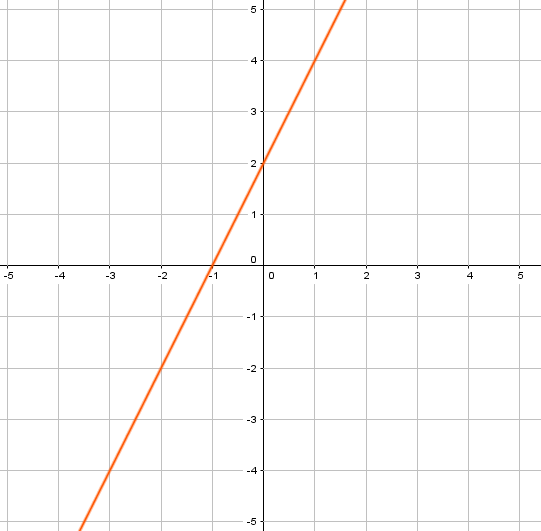
\includegraphics[scale=0.5]{ex1}
			\end{column}			
			
		\end{columns}
	\end{myex}
\end{frame}

\subsection{Sens de variation}

\begin{frame}

\begin{myprop}
	Le sens de variation d'une fonction affine dépend du signe de $a$ :
	\begin{itemize}
		\item Si \kw{$a > 0$}, la droite \kw{"monte"}, la fonction est \kw{croissante};
		\item Si \kw{$a < 0$}, la droite \kw{"descend"} la fonction est \kw{décroissante};
		\item Si \kw{$a = 0$}, la droite est \kw{horizontale}, la fonction est \kw{constante}.
	\end{itemize}
\end{myprop}

\end{frame}


\begin{frame}
	%\frametitle{Exemples}

	\begin{myex}
		$f, g$ et $h$ sont des fonctions affines telles que :
	\end{myex}
	
	\begin{columns}[c]
		
		
		\begin{column}{3.7cm}
			
			\begin{exampleblock}{$f(x)=2x+1$}
				
				
				\begin{center}
					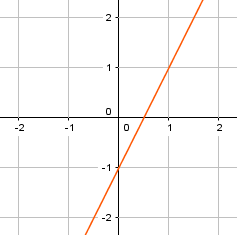
\includegraphics[scale=0.5]{ex2_1}
				\end{center}		
				
				$a=2$; $a>0$, la droite "monte", la fonction est croissante. 	
			\end{exampleblock}
			
		\end{column}
		
		\begin{column}{3.7cm}
			\begin{exampleblock}{$g(x)=-x+1$}
			
				\begin{center}
					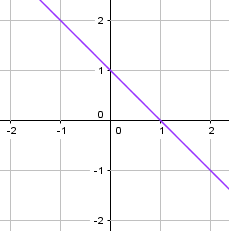
\includegraphics[scale=0.5]{ex2_2}
				\end{center}		
			
				$a=-1$; $a<0$, la droite "descend", la fonction est décroissante. 
			\end{exampleblock}
		\end{column}
		
		\begin{column}{3.7cm}
			\begin{exampleblock}{$h(x)=3$}
			
				\begin{center}
					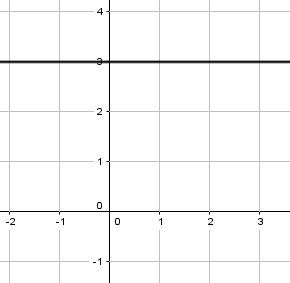
\includegraphics[scale=0.45]{ex2_3}
				\end{center}		
				$a=0$, la droite est horizontale, la fonction est constante. 
			\end{exampleblock}
		\end{column}
	
	\end{columns}



\end{frame}

\subsection{Calcul du coefficient directeur}


\begin{frame}
	\begin{mymeth}
		Pour calculer le coefficient directeur d'une fonction affine $f$, on a besoin de deux nombres distincts $x_1$ et $x_2$ et de leurs images par $f$, $f(x_1)$ et $f(x_2)$. On a alors :

		\kw{\begin{align*}
			a = \dfrac{f(x_2) - f(x_1)}{x_2 - x_1}
		\end{align*}}
	\end{mymeth}
\end{frame}	

\begin{frame}
	\begin{myex}
		La fonction passe par les points de coordonnées $(2;4)$ et $(4;8)$, on a :
		
		\begin{align*}
		a &= \frac{8-4}{4-2} \\
		a &= \frac{4}{2} \\
		a &= 2
		\end{align*}
	\end{myex}
	
\end{frame}

\end{document}